\section{The Large Hadron Collider at CERN}%
\label{sec:lhc}

The LHC~\cite{Evans:2008zzb} is a particle collider experiment located at
CERN\footnote{From the French \emph{Conseil Européen pour la Recherche
    Nucléaire} referring to both the research organisation and the location of
  the laboratory sites.} at the French--Swiss border in Geneva, Switzerland.  At
present, the LHC is the world's highest-energy, laboratory-based particle
collider experiment accelerating protons to energies of up to \SI{6.8}{\TeV}
resulting in proton--proton (\pp) centre-of-mass energies, $\sqrt{s}$, of up to
\SI{13.6}{\TeV}. The LHC is also used to accelerate heavy-ions, however, the
focus of this section lies in the operation of the LHC in \pp-collison mode, the
analysis of \pp~collision data being the subject of this thesis.

The LHC was constructed in the former tunnel of the CERN Large Electron-Positron
Collider (LEP) with a circumference of \SI{26.7}{\kilo\metre} and became first
operational in 2008. It is a synchrotron consisting of two counter-rotating
beams of protons that are accelerated using alternating electric fields in
superconducting radio frequency resonators. The beams are bent into a cyclic
trajectory around the LHC ring using superconducting dipole magnets with field
strengths of about \SI{8}{\tesla}. Along the ring, numerous quadrupole magnets
are used for controlled focusing and defocusing of the proton beams.
% Synchrotron: 1232 dipoles (superconducting) -> Magnetic field of
% \SI{8.3}{\tesla} required for \SI{7}{\TeV} beam energy operation
The proton beams consist of localised packages of ca.\ $10^{11}$ protons,
hereafter referred to as bunches, circulating in the LHC with a minimum spacing
in time of \SI{25}{\nano\second}~\cite{Evans:2008zzb}.

The proton energies necessary for the injection into the LHC are achieved using
a sequence of particle accelerators at CERN, schematically depicted
in~\Cref{fig:cern_accelerator_complex}. Protons are first accelerated in LINAC 2
after which they pass through the Proton Synchrotron Booster (BOOSTER), the
Proton Synchrotron (PS), and the Super Proton Synchrotron (SPS). The SPS
accelerates protons to an energy of \SI{450}{\GeV}~\cite{Evans:2008zzb},
subsequently injecting the protons into the LHC. In the LHC, the protons are
further accelerated until the target energy is reached. Afterwards, the beams
are brought into collision at four points, the interaction points (IPs), along
the ring. Four large experiments are situated at the IPs to observe and record
particle collision events: ATLAS~\cite{PERF-2007-01}, CMS~\cite{CMS-CMS-00-001},
ALICE~\cite{ALICE:2008ngc}, and LHCb~\cite{LHCb:2008vvz}. The ATLAS and CMS
experiments are particle detector experiments targeting largely overlapping,
extensive physics programmes, while the ALICE and LHCb adopt more specialised
programmes. The ALICE experiment studies the production of the quark-gluon
plasma, a state of matter with asymptotically free quarks and gluons occurring
at temperatures similar to those right after the Big Bang, in heavy-ion
collisions. The LHCb experiment investigates the nature the matter-antimatter
asymmetry in the universe by studying CP violation in decays of hadrons
containing $b$-quarks. Several smaller experiments are installed at the LHC to
study physics processes at small angles with respect to the LHC beamline or
search for exotic particles. These experiments are LHCf~\cite{LHCf:2008lfy},
TOTEM~\cite{TOTEM:2008lue}, and MoEDAL~\cite{MoEDAL:2009jwa}.\footnote{For the
  data-taking period starting in 2022, two additional experiments called
  FASER~\cite{FASER:2019aik} and SND@LHC~\cite{Boyarsky:2021moj} were
  comissioned.}


\begin{figure}[htbp]
  \centering

  %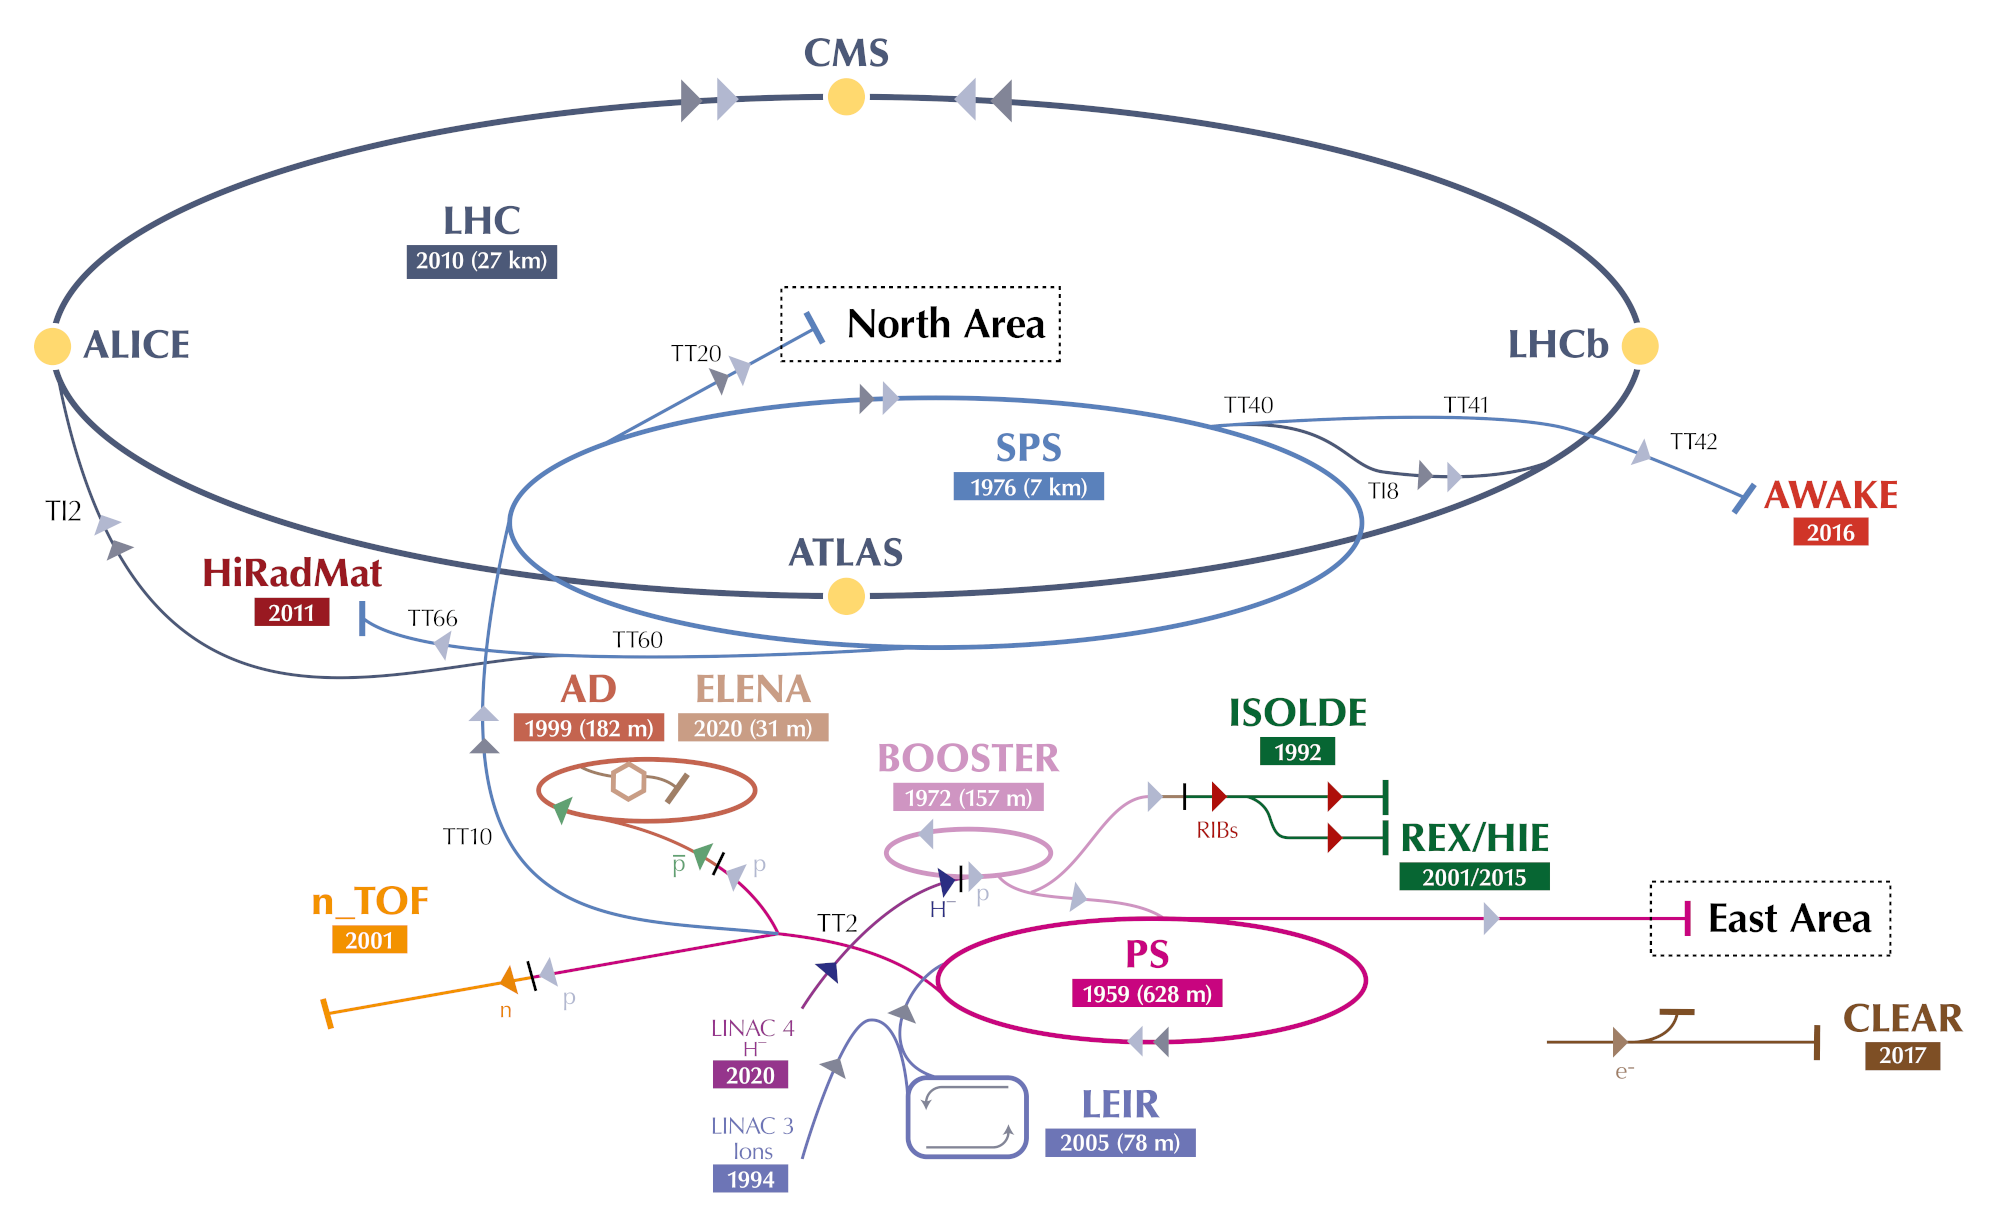
\includegraphics[width=0.9\textwidth, trim=10.5cm 44cm 2cm 20cm,
  %clip]{lhc/cern_complex}
  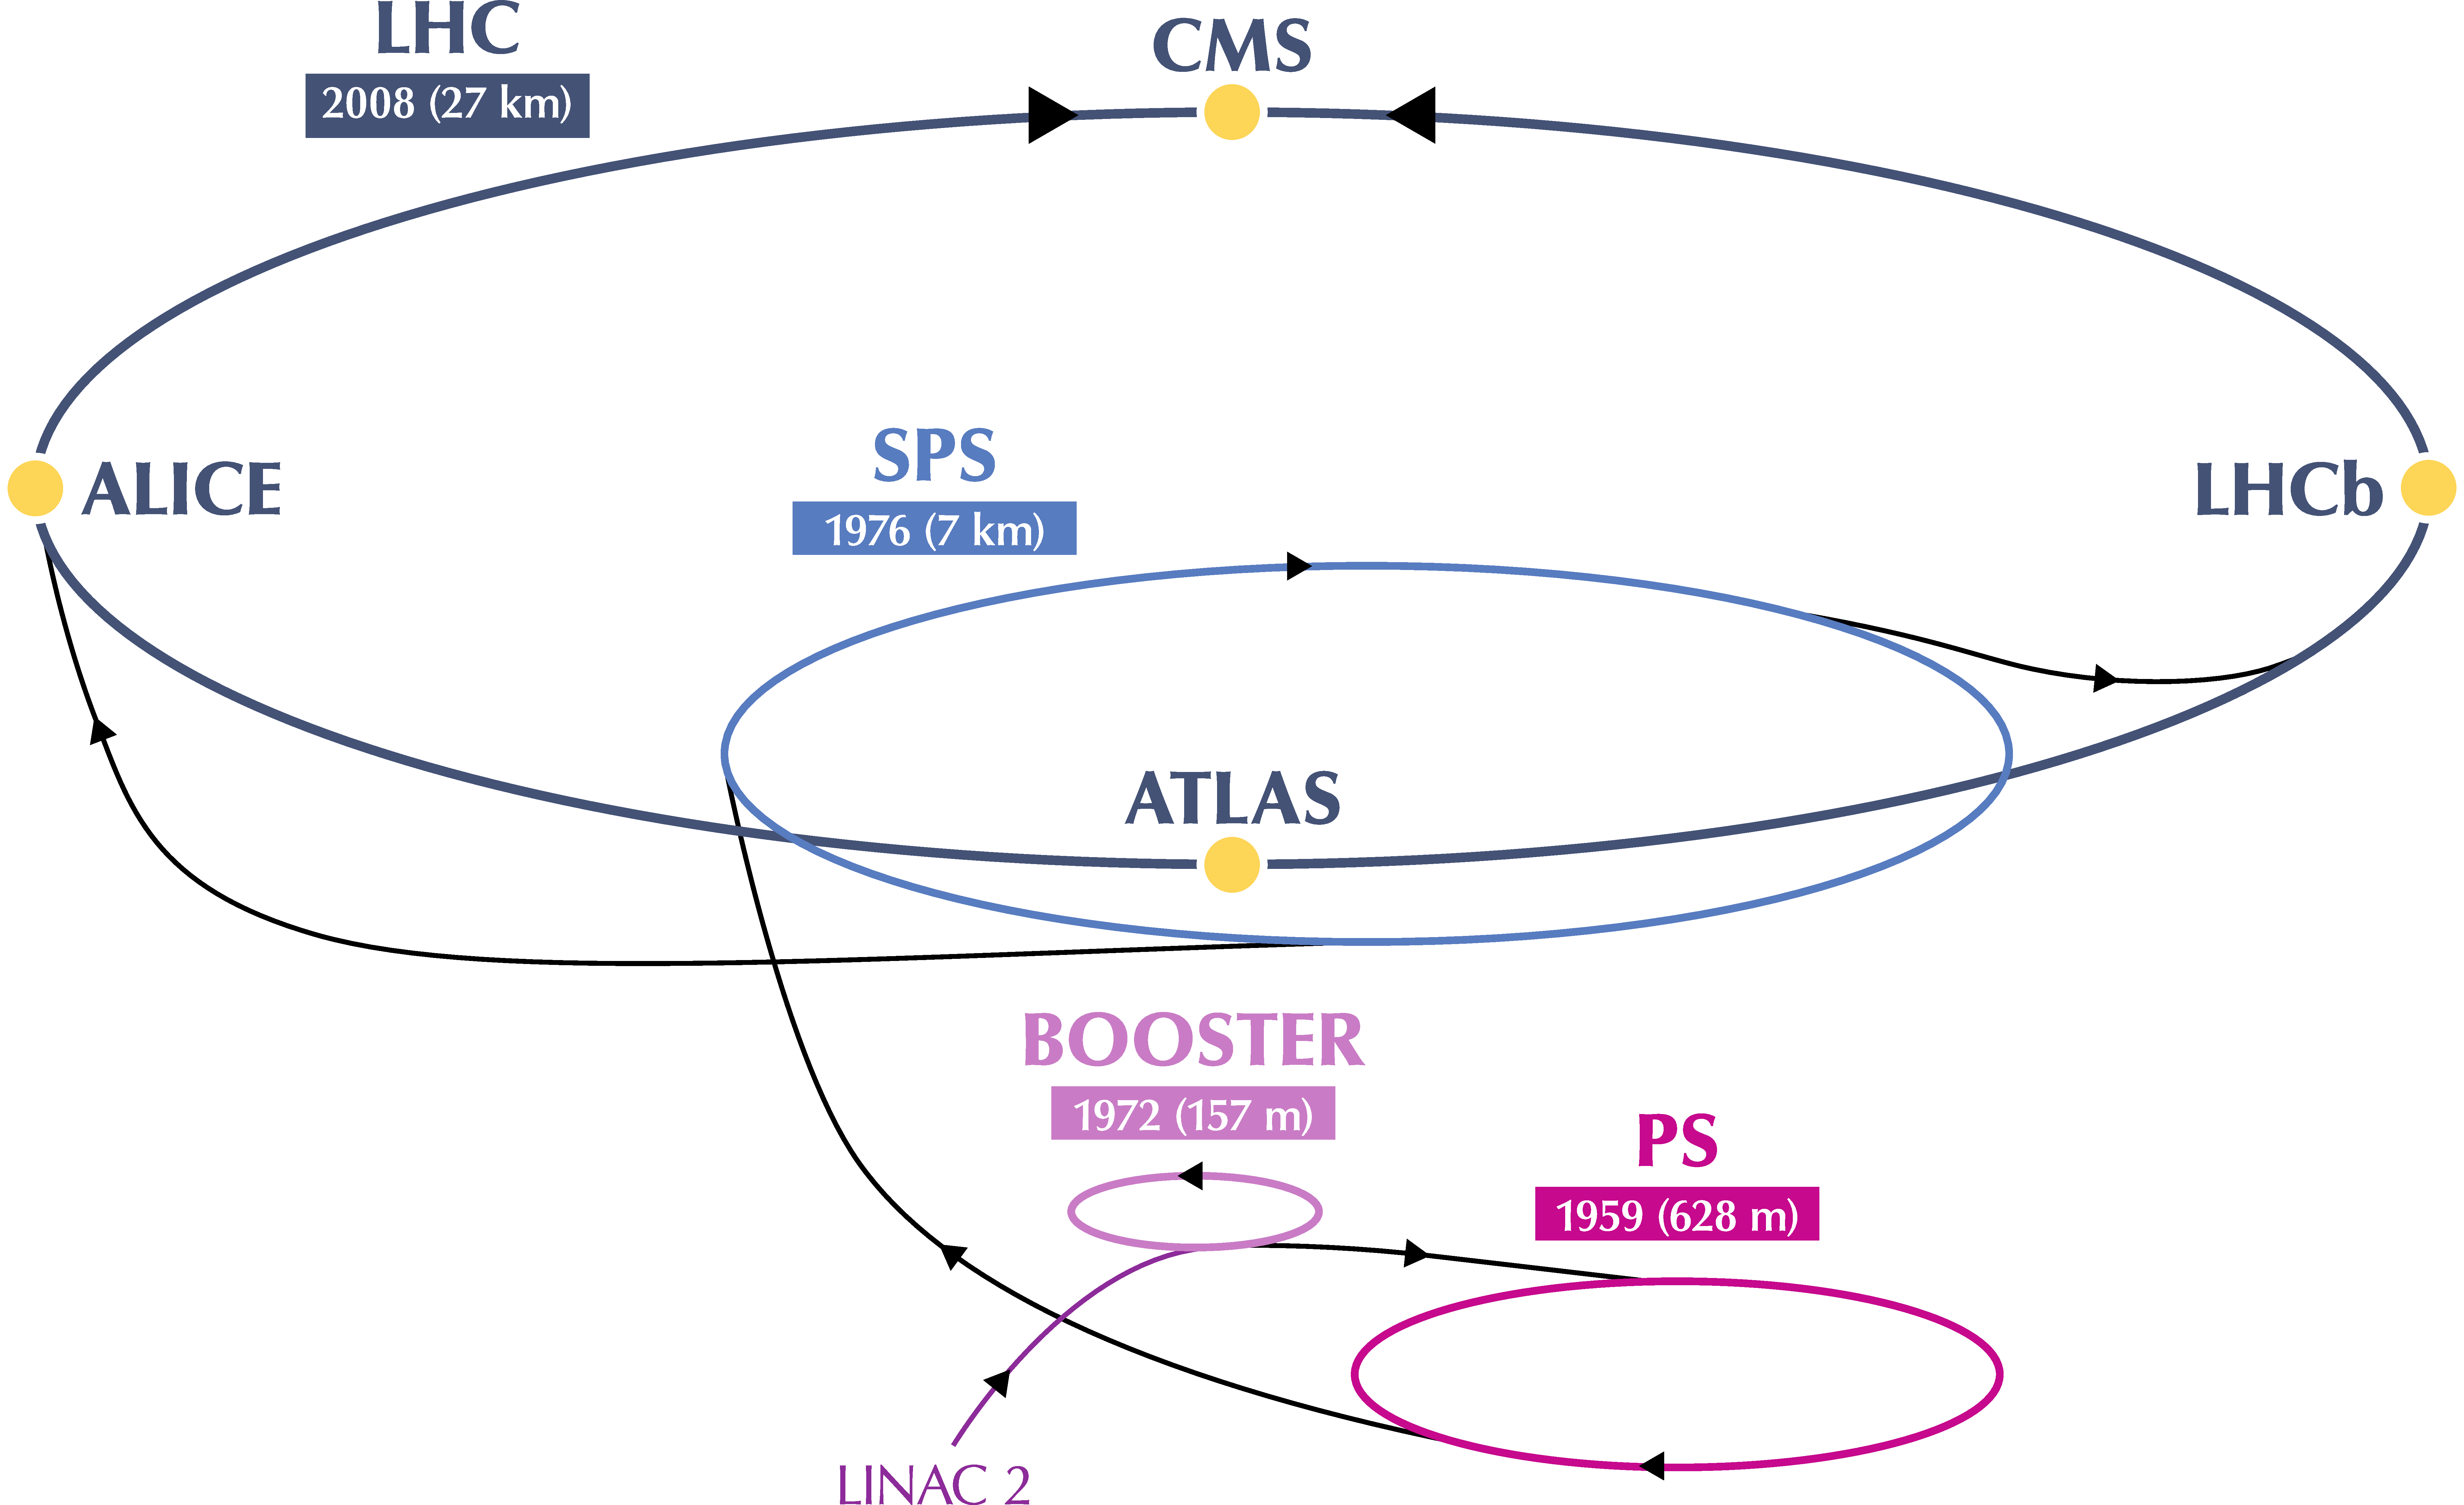
\includegraphics[width=0.75\textwidth]{lhc/cern_complex_trim_otherexp_removed}

  \caption[Illustration of the LHC and its pre-accelerators.]{Illustration of
    the LHC and its pre-accelerators when operating in proton--proton collision
    mode during the data-taking period from 2015--2018 (Run~2). The year of
    first operation and circumference of the accelerators is given in solid
    coloured boxes. The figure is adapted from Ref.~\cite{Mobs:2684277}.}%
  \label{fig:cern_accelerator_complex}
\end{figure}

The main operating period of the LHC started in 2010 with \pp~collisions at
$\sqrt{s} = \SI{7}{\TeV}$. In 2012, the centre-of-mass energy was increased to
\SI{8}{\TeV}. The data-taking period from 2010 to 2012 is referred to as
\emph{Run~1} of the LHC. After extensive upgrades of the LHC and the detectors,
the LHC restarted operation with \pp~collisions at $\sqrt{s} = \SI{13}{\TeV}$ in
\emph{Run~2} which took place from 2015 to 2018. After another shutdown of LHC
and experiments, data-taking recommenced in 2022 with \emph{Run~3}, reaching
unprecedented energy scales of $\sqrt{s} = \SI{13.6}{\TeV}$. At present, Run~3
is foreseen to last until the end of 2025~\cite{lhc_schedule}.

An important performance characteristic of a particle collider is the
instantaneous luminosity, $L$, at a given interaction point. For a process $p$,
the instantaneous luminosity relates the expected number of events from the
process per unit time, $\mathrm{d}N_{p} / \mathrm{d}t$, to the cross section of
the process, $\sigma_{p}$, according to
\begin{align*}
  \frac{\mathrm{d}N_{p}}{\mathrm{d}t} = L \sigma_{p} \,\text{.}
\end{align*}
The expected number of events over a time interval, assuming constant
cross section, is given by $N_{p} = L_{\text{int}} \, \sigma_{p}$, where
$L_{\text{int}} = \int \mathrm{d}t \, L(t)$ is referred to as the integrated
luminosity. When searching for rare physics processes occuring at high-energy
scales, it is typically desirable to perform collisions at the largest,
experimentally feasible $L$ over extensive time periods to maximise the expected
number of events from the rare process.

The integrated luminosity delivered to the ATLAS experiment by the LHC during
Run~2 is shown in \Cref{fig:atlas_int_lumi_vs_time}. In this data-taking period,
the LHC delivered \pp~collisions with an integrated luminosity of about
\SI{156}{\per\femto\barn} of which \SI{139}{\per\femto\barn} pass the
data-quality requirements of the ATLAS experiment~\cite{ATLAS-CONF-2019-021}.
The peak instantaneous luminosity at the IP of the ATLAS experiment ranged from
\SI{0.5e-34}{\per\centi\metre\squared\per\second} at the beginning, to
\SI{1.9e-34}{\per\centi\metre\squared\per\second} at the end of the
Run~2~\cite{ATLAS-CONF-2019-021}. A quantity related to the instantaneous
luminosity is the expected number of inelastic \pp interactions per bunch
crossing, $\mu$. Due to the large cross section of inelastic \pp~collisions at
$\sqrt{s} = \SI{13}{\TeV}$ of about \SI{80}{\milli\barn}~\cite{STDM-2015-05},
multiple interactions occur in a single crossing of the proton bunches. These
interactions contaminate collision events of interest and are referred to as
pile-up. The distribution of $\mu$ is depicted in \Cref{fig:atlas_mu} at the IP
at the ATLAS experiment during Run~2, showing that on average \num{33.7}
inelastic collision events are expected to occur in a single bunch crossing in
the combined Run~2 \pp~collision dataset.

% Luminosity or pile-up plots?
% https://twiki.cern.ch/twiki/bin/view/AtlasPublic/LuminosityPublicResultsRun2

\begin{figure}[htbp]
  \centering

  \begin{subfigure}{0.47\textwidth}
    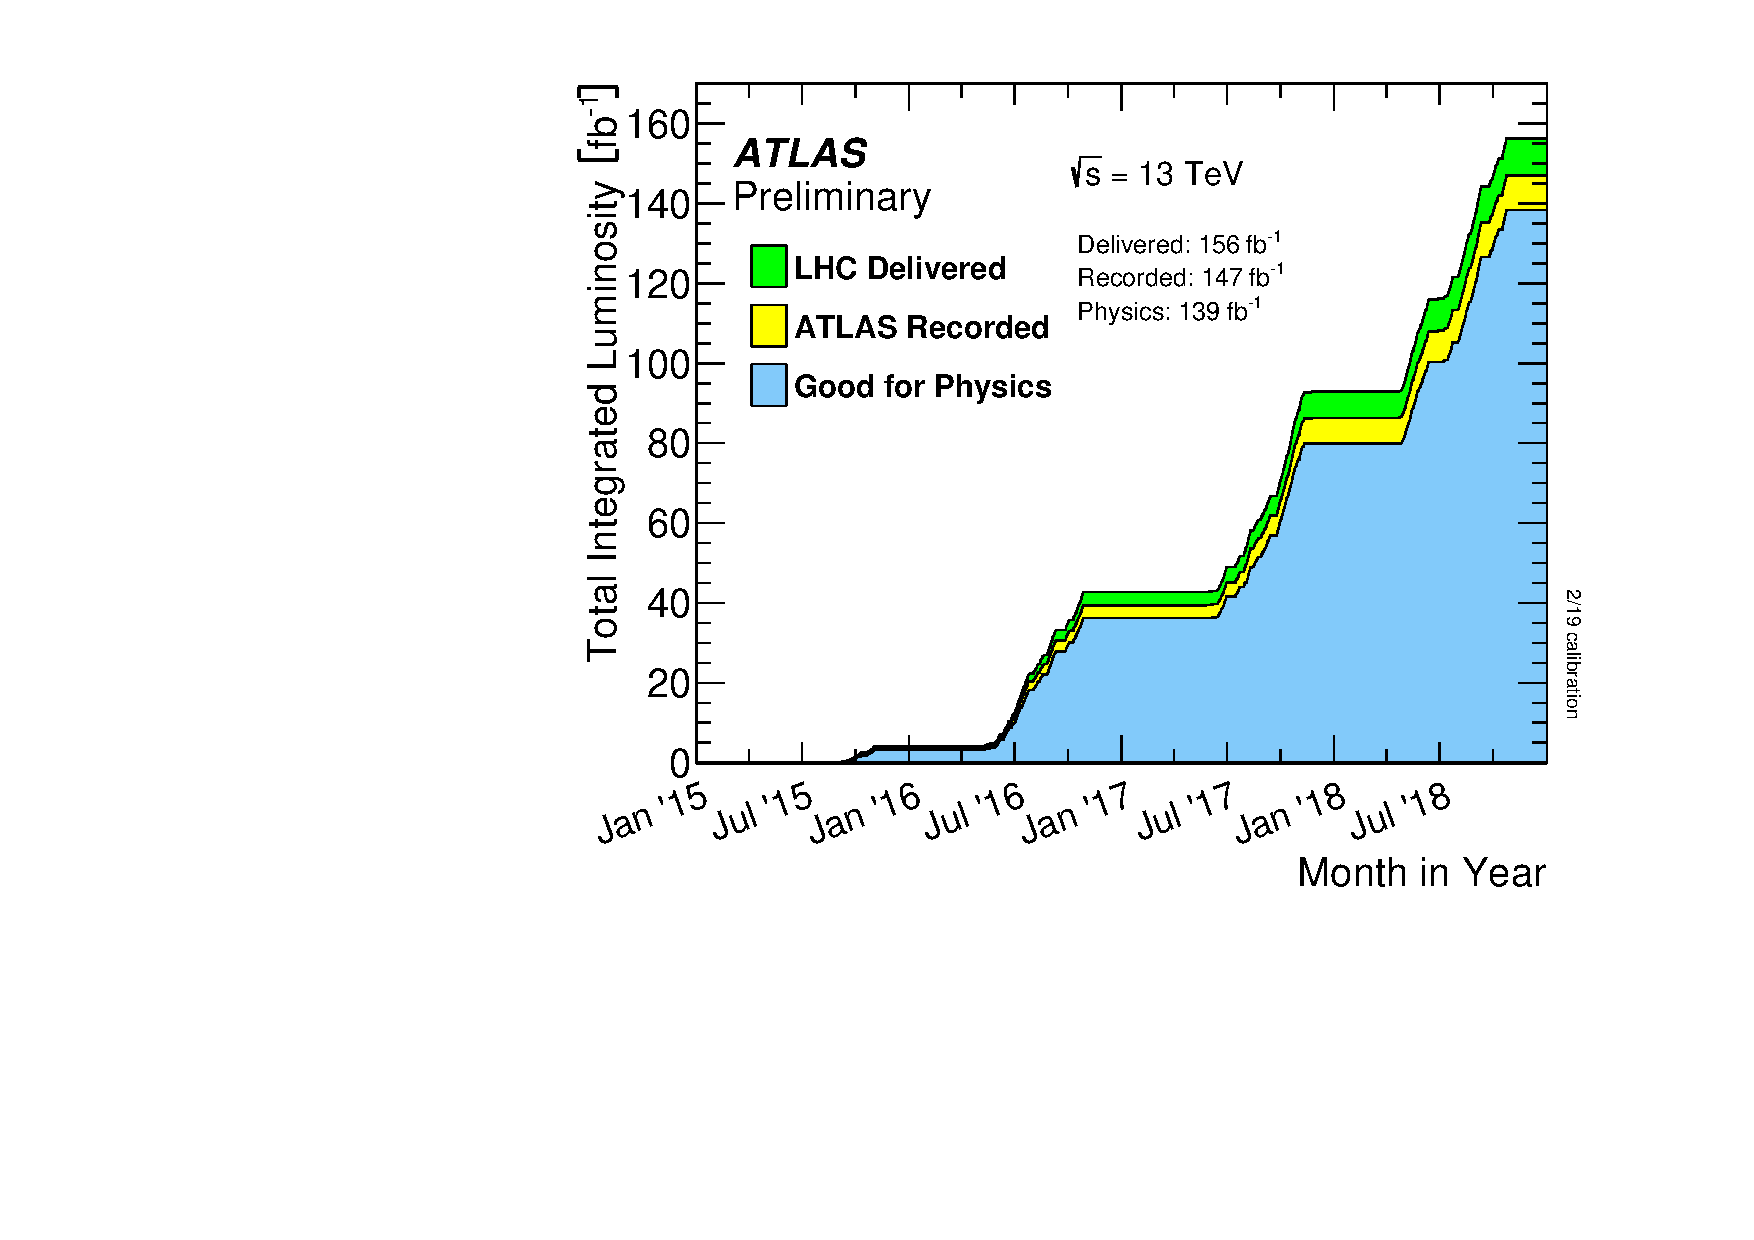
\includegraphics[width=\textwidth]{lhc/int_lumi_vs_time}
    \subcaption{}%
    \label{fig:atlas_int_lumi_vs_time}
  \end{subfigure}\hspace*{0.02\textwidth}%
  \begin{subfigure}{0.47\textwidth}
    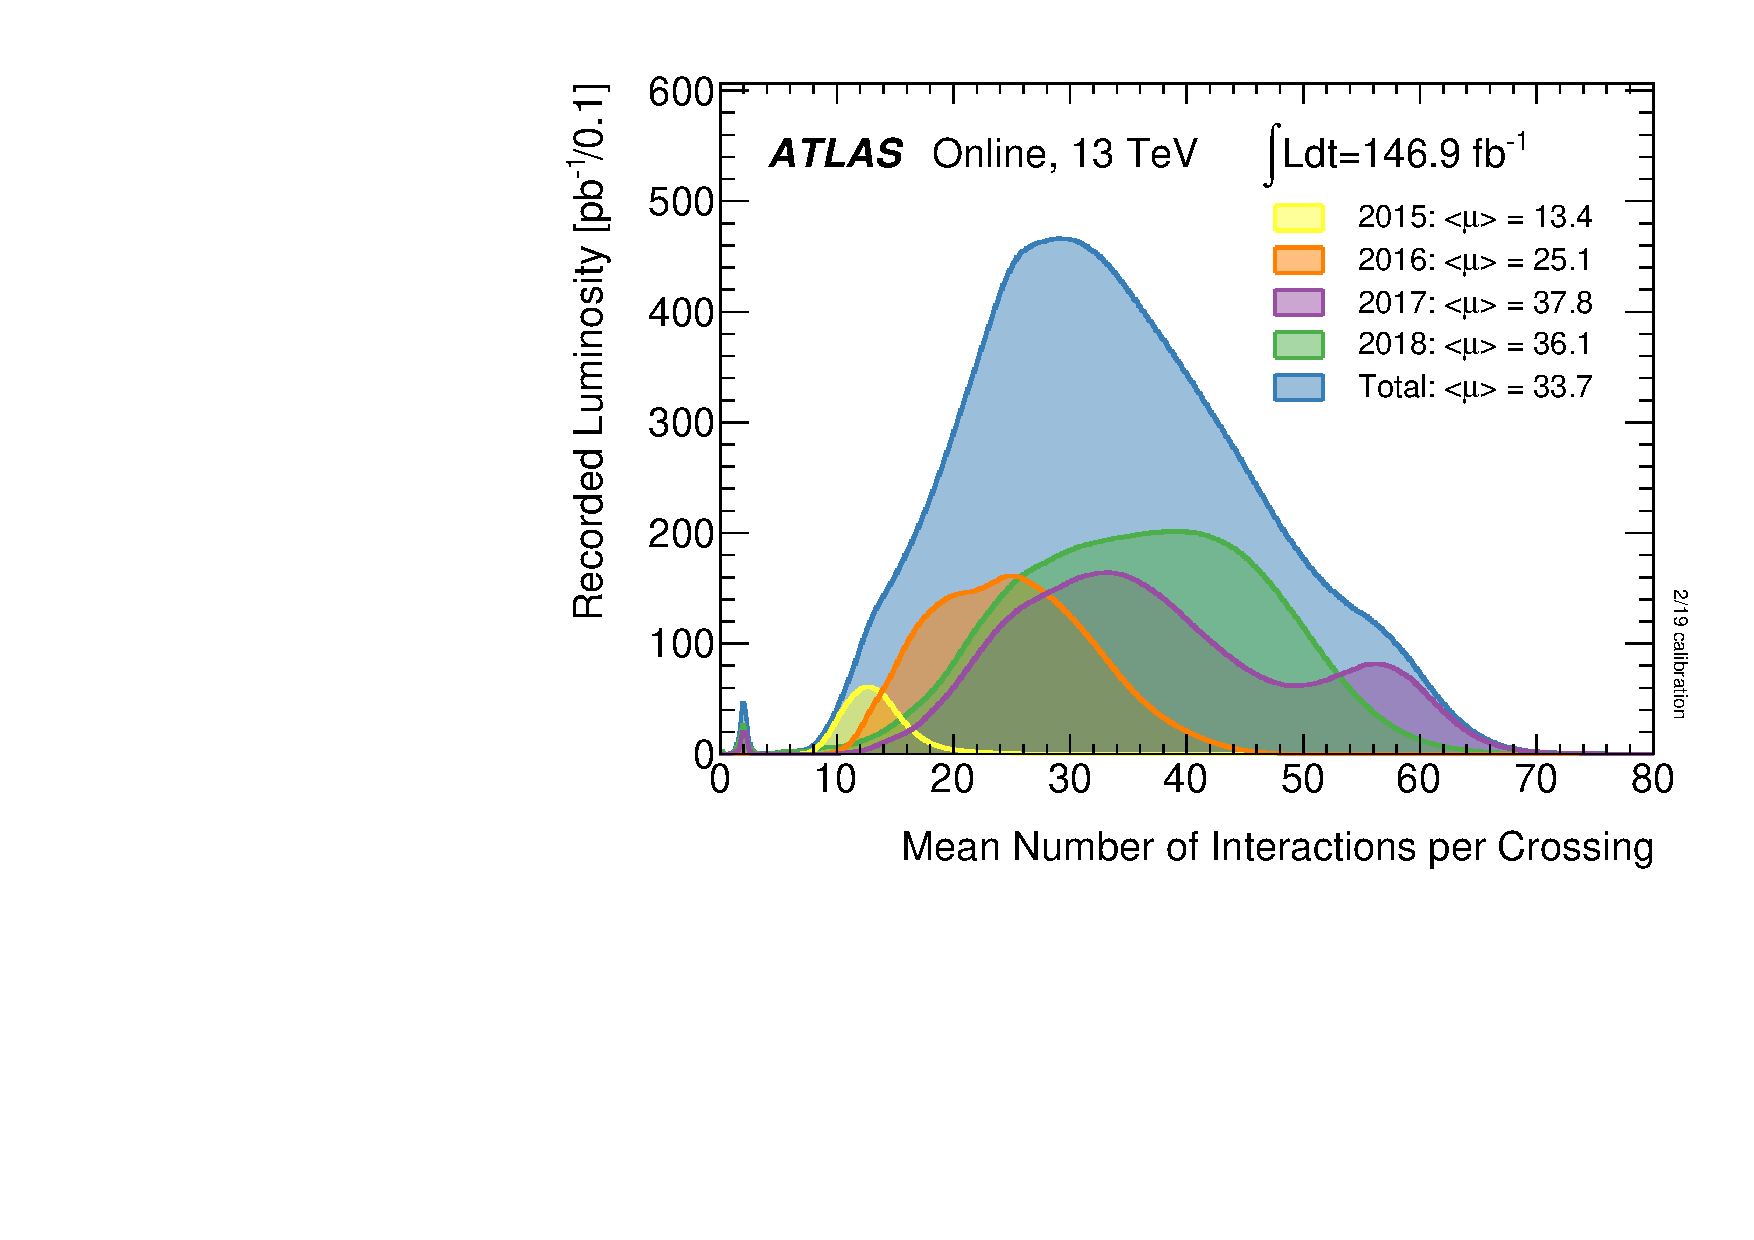
\includegraphics[width=\textwidth]{lhc/mu_2015_2018}
    \subcaption{}%
    \label{fig:atlas_mu}
  \end{subfigure}

  \caption[The integrated luminosity and the mean number of interactions per
  bunch crossing at the ATLAS experiment during Run~2 of the LHC.]{The
    integrated luminosity as a function of time (a) and the distribution of the
    mean number of interactions per bunch crossing (b) of the LHC in \pp
    operation mode during Run~2. In Figure (a), the integrated luminosity
    delivered by the LHC (green), recorded by the ATLAS detector (yellow), and
    passing the data-quality criteria~\cite{DAPR-2018-01} of the ATLAS
    collaboration (blue) is shown. In Figure (b), the mean number of
    interactions per bunch crossing is calculated from the instantaneous
    luminosity assuming an inelastic \pp~collision cross section at
    $\sqrt{s} = \SI{13}{\TeV}$ of \SI{80}{\milli\barn}. The figures are taken
    from Ref.~\cite{atlas_luminosity_summary_plots}.}%
  \label{fig:lumi_and_pu}
\end{figure}

%%% Local Variables:
%%% mode: latex
%%% TeX-master: "../../phd_thesis"
%%% End:
